\documentclass{article}
\usepackage{graphicx}
\usepackage[a4paper, total={6in, 8in}]{geometry}

\title{Graph Theory Coursework}
\author{Jay Drinkwater}
\date{December 2026}

\begin{document}

\maketitle

\begin{figure}[h!]
  \begin{center}
    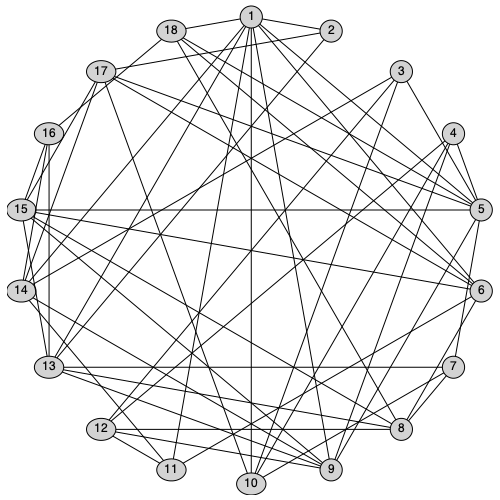
\includegraphics[width=0.9\textwidth]{./My Graph.png}
  \end{center}
  \label{fig:graph}
\end{figure}

\newpage

\section{Introduction}

To start, I will be referring to my personal graph as [Graph Name],


\section{Adjacencies and Degrees of Vertices}

\subsection{Adjacencies}
An adjacent vertex, $y$, to a vertex, $x$, is a vertex such that there is an edge connecting $x$ to $y$.
\flushleft
The following table lists the adjacent vertices for each vertex $k \in [1,18]$.

\begin{table}[h!]
  \begin{center}
    \begin{tabular}{|c||l|}
    \hline
    
      Vertex, $k$   & Adjacent Vertices \\

    \hline
    \hline

      1 & 2, 5, 6, 9, 10, 11, 13, 14, 18 \\
        \hline
      2 & 1, 13, 17  \\
      \hline
      3 & 5, 10, 12, 14 \\
      \hline
      4 & 5, 9, 10, 12 \\
      \hline
      5 & 1, 3, 4, 7, 9, 15, 17, 18 \\
      \hline
      6 & 1, 8, 11, 15, 17, 18 \\
      \hline
      7 & 5, 8, 10, 13 \\
      \hline
      8 & 6, 7, 12, 13, 15, 18 \\
      \hline
      9 & 1, 4, 5, 12, 13, 14, 15  \\
      \hline
      10 & 1, 3, 4, 7, 17  \\
      \hline
      11 & 1, 6, 12, 14  \\
      \hline
      12 & 3, 4, 8, 9, 11 \\
      \hline
      13 & 1, 2, 7, 8, 9, 15, 16 \\
      \hline
      14 & 1, 3, 9, 11, 16, 17  \\
      \hline
      15 & 5, 6, 8, 9, 13, 16, 17 \\
      \hline
      16 & 13, 14, 15, 18 \\
      \hline
      17 & 2, 5, 6, 10, 14, 15 \\
      \hline
      18 & 1, 5, 6, 8, 16 \\
      \hline
    \end{tabular}
  \end{center}
\label{tab:adjacent vertices}
\end{table}


\subsection{Degrees of Vertices}
Definition: the degree of a vertex $x$, $deg(x)$ is the number of edges leaving that vertex.
\flushleft
Now, from the table above containing all edges leaving each vertex, we can use the definition of the degree of a vertex to find the degree of every vertex $k \in [1,18]$ for [Graph Name]. This is what the table below does.
\flushleft
Also to note, $\Delta ([Graph Name])$ means the maximum degree of [Graph Name], this is just the vertex/vertices with the largest degree. [Graph Name] only has the maximum degree at 1 vertex, vertex 1. This is because $deg(1) = 9 \geq k$ where $k \in [1,18]$
\flushleft
Similarly, $\delta ([Graph Name])$ means the minimum degree of [Graph Name], which also only occurs at a single vertex, vertex 2, as $deg(2) = 3 \leq deg(k)$ where $k \in [1,18]$.
\flushleft
A unique vertex, as suggested by the name, is a vertex where no other vertices in the graph have the specified property, like with vertex 1, it is a unique vertex with degree 9 as no other vertices have degree 9.

\begin{table}[h!]
  \begin{center}
    \begin{tabular}{|c||c|c|c|c|c|c|c|c|c|c|c|c|c|c|c|c|c|c|}
    \hline
      Vertex & 1&2&3&4&5&6&7&8&9&10&11&12&13&14&15&16&17&18 \\
      \hline
      Edges & 9&3&4&4&8&6&4&6&7&5&4&5&7&6&7&4&6&5 \\
      \hline
    \end{tabular}
  \end{center}
\label{tab:degrees of vertices horizontal}
\end{table}


\section{Edges}
Below is a table containing all 49 MAYBE FIFTY??? edges in [Graph Name]. Each edge is only listed once as $1 \cdot 2 = 2 \cdot 1$ and so on.
\begin{table}[ht!]
  \begin{center}
    \begin{tabular}{|c||r|r|r|r|r|r|r|r|r|}
    \hline
    
    \hline

      1 & $1 \cdot2$ & $1 \cdot5$ & $1 \cdot6$ & $1 \cdot9$ & $1 \cdot10$ & $1 \cdot11$ & $1 \cdot13$ & $1 \cdot14$ & $1 \cdot18$ \\
        \hline
      2 & $2 \cdot13$ & $2 \cdot17$ & & & & & & &  \\
      \hline
      3 & $3 \cdot5$ & $3 \cdot10$ & $3 \cdot12$ & $3 \cdot14$ &&&&&   \\
      \hline
      4 & $ 4\cdot5$ & $4 \cdot9$ & $4 \cdot10$ & $4 \cdot12$ &&&&&  \\
      \hline
      5 & $5 \cdot7$ & $5 \cdot9$ & $5 \cdot15$ & $5 \cdot17$ & $5 \cdot18$ &&&&  \\
      \hline
      6 & $6 \cdot8$ & $6 \cdot11$ & $6 \cdot15$ & $6 \cdot17$ & $6 \cdot18$ &&&&  \\
      \hline
      7 & $7 \cdot8$ & $7 \cdot10$ & $7 \cdot13$ &&&&&& \\
      \hline
      8 & $8 \cdot12$ & $8 \cdot13$ & $8 \cdot15$ & $8 \cdot18$ &&&&& \\
      \hline
      9 & $9 \cdot12$ & $9 \cdot13$ & $9 \cdot14$ & $9 \cdot15$ &&&&& \\
      \hline
      10 & $10 \cdot17$ &&&&&&&& \\
      \hline
      11 & $11 \cdot14$ &&&&&&&& \\
      \hline
      13 & $13 \cdot15$ & $13 \cdot16$ &&&&&&& \\
      \hline
      14 & $14 \cdot16$ & $14 \cdot17$  &&&&&&& \\
      \hline
      15 & $15 \cdot16$ & $15 \cdot17$ &&&&&&& \\
      \hline
      16 & $16 \cdot18$ &&&&&&&& \\
      \hline

    \end{tabular}
  \end{center}
\label{tab:edges}
\end{table}



\section{Bipartite-ness}

\noindent
\begin{minipage}{0.4\textwidth}
    To the right are a few examples of the triangles in [Graph Name] \\
    Take, for example, the red triangle, it has vertices 4, 9, and 12. By Lemma 2.3.0.4, as [Graph Name] has three distinct pairwise adjacent vertices, [Graph Name] is not bipartite. \\
\end{minipage}
\hspace{1cm}
\begin{minipage}{0.4\textwidth}
    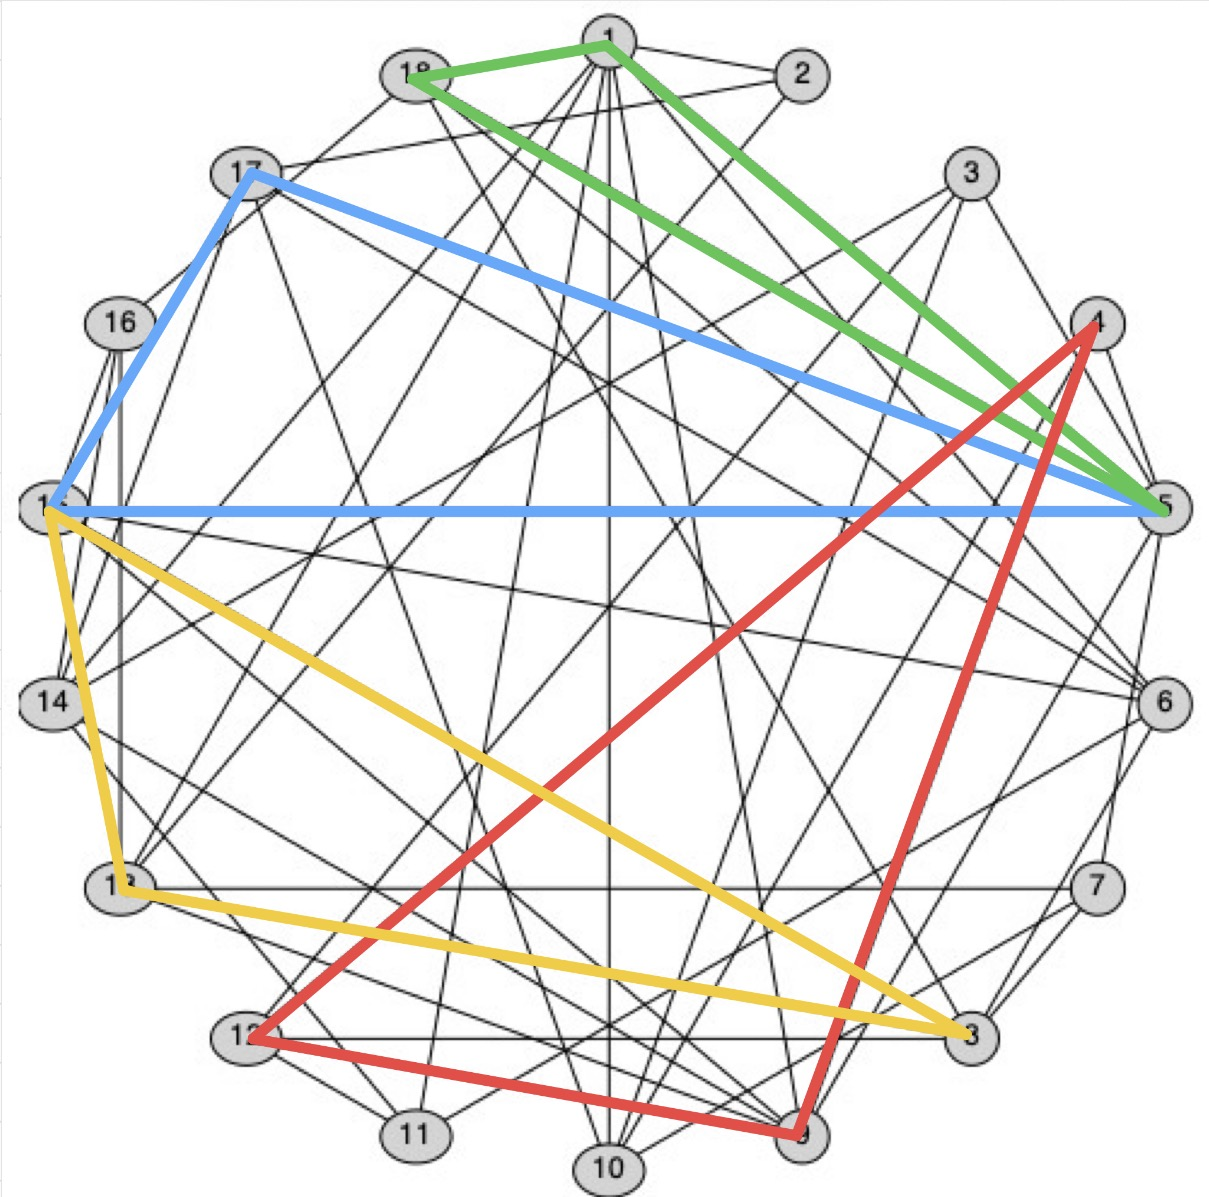
\includegraphics[width=\linewidth]{Graph with triangles.png}
\end{minipage}
\hfill


\end{document}